\documentclass[final,hyperref={pdfpagelabels=false}]{beamer}
\mode<presentation>{\usetheme{Insight}}

% To install ubuntu fonts in LaTeX:
% https://github.com/tzwenn/ubuntu-latex-fonts
%
\usepackage{ubuntu}

% Set Size of poster with size= property: a1, a2, a3 debug
\usepackage[orientation=portrait,size=a0,scale=1.4]{beamerposter}

% Required Packages:
\usepackage{amsmath,amsthm, amssymb, latexsym}
%\boldmath
\usepackage[english]{babel}
\usepackage[utf8]{inputenc}
\usepackage{tikz}
\usepackage{graphics}
\usepackage{overpic}
\usepackage{ragged2e}
\usepackage{tcolorbox}
\tcbuselibrary{skins}
\usetikzlibrary{shadings}
\usepackage{tikz}
\usetikzlibrary{positioning}
\usepackage{tikz}
\usepackage{colortbl}
\usepackage{longtable}
\usepackage{qrcode}
\usepackage{subfigure}

\usepackage{booktabs}
\usepackage{multirow}
\usepackage{multicol}
\setlength\columnsep{1.4cm}



%%%% replace as required
\title{\huge \textbf{A Tool to Build and Rank Literature Surveys}}
\author{Helmut Simonis and Cemalettin Öztürk}
\institute[Insight]{Insight SFI Centre for Data Analytics\\School of Computer Science and Information Technology\\University College Cork\\Cork, Ireland}

\date{}
%%%%%%%%%%%%%%%%%%%%%%%%%%%%%%%%%%%%%%%%%%%%%%%%%%%%%%%%%%%%%%%%%%%%%%%%%%%%%%
\begin{document}
\begin{frame}{}
%%%%%%%%%%%%%%%%%%%%%%%%%%%%%%%%%%%%%%%%%%%%%%%%%%%%%%%%%%%%%%%%%%%%%%%%%%%%%%

\begin{multicols}{2}

\section{Problem}
\begin{itemize}
\item A comprehensive and accurate literature survey is required for any project we undertake
\item Using standard bibliographic search tools can be inaccurate, needing manual filtering (up to 90\% misses)
\item Manual search is error prone and time consuming, often misses relevant work
\item A tool is needed to help find, classify, and rank relevant literature
\end{itemize}

\section{Assumptions}
\begin{itemize}
\item All relevant works in an area are connected by either citations or references
\item We need to find works in journal \emph{and} proceedings
\item Any recent work will have a DOI as identifier
\item Combination of different search end-points will provide most of required information
\begin{itemize}
\item OpenCitations, Scopus, Crossref, (WoS)
\item No search engine provides all required information
\end{itemize} 
\item \emph{Human in the loop}, not fully automatic
\end{itemize}

\section{Process}

{\centering
\begin{tikzpicture}[xscale=6,yscale=5]
\node[draw=black,fill=pantone_127_4,rounded corners] (bib) at (2,4) {Bib File};
\node[draw=black,fill=pantone_157_8,rounded corners] (refs) at (1,3) {\shortstack{References\\Citations}};
\node[draw=black,fill=pantone_10_7,rounded corners] (works) at (2,2) {PDF};
\node[draw=black,fill=pantone_157_8,rounded corners] (concepts) at (3,3) {\shortstack{Extracted\\Concepts}};
\node[draw=black,fill=pantone_119_1,rounded corners] (reports) at (2,1) {Reports};
\draw[very thick,black,->] (bib) -- node[left] {Using REST services} (refs);
\draw[very thick,black,->] (refs) -- node[left] {Manual} (works);
\draw[very thick,black,->] (refs) -- node[above] {\shortstack{Title\\Abstract\\Keywords}} (concepts);
\draw[very thick,black,->] (works) -- node[right] {as LaTeX} (reports);
\draw[very thick,black,->] (works) -- node[right] {pdfgrep} (concepts);
\draw[very thick,black,->] (concepts) -- node[right] {Add relevant works} (bib);
\end{tikzpicture}
}


\section{Bibliometric Overview}

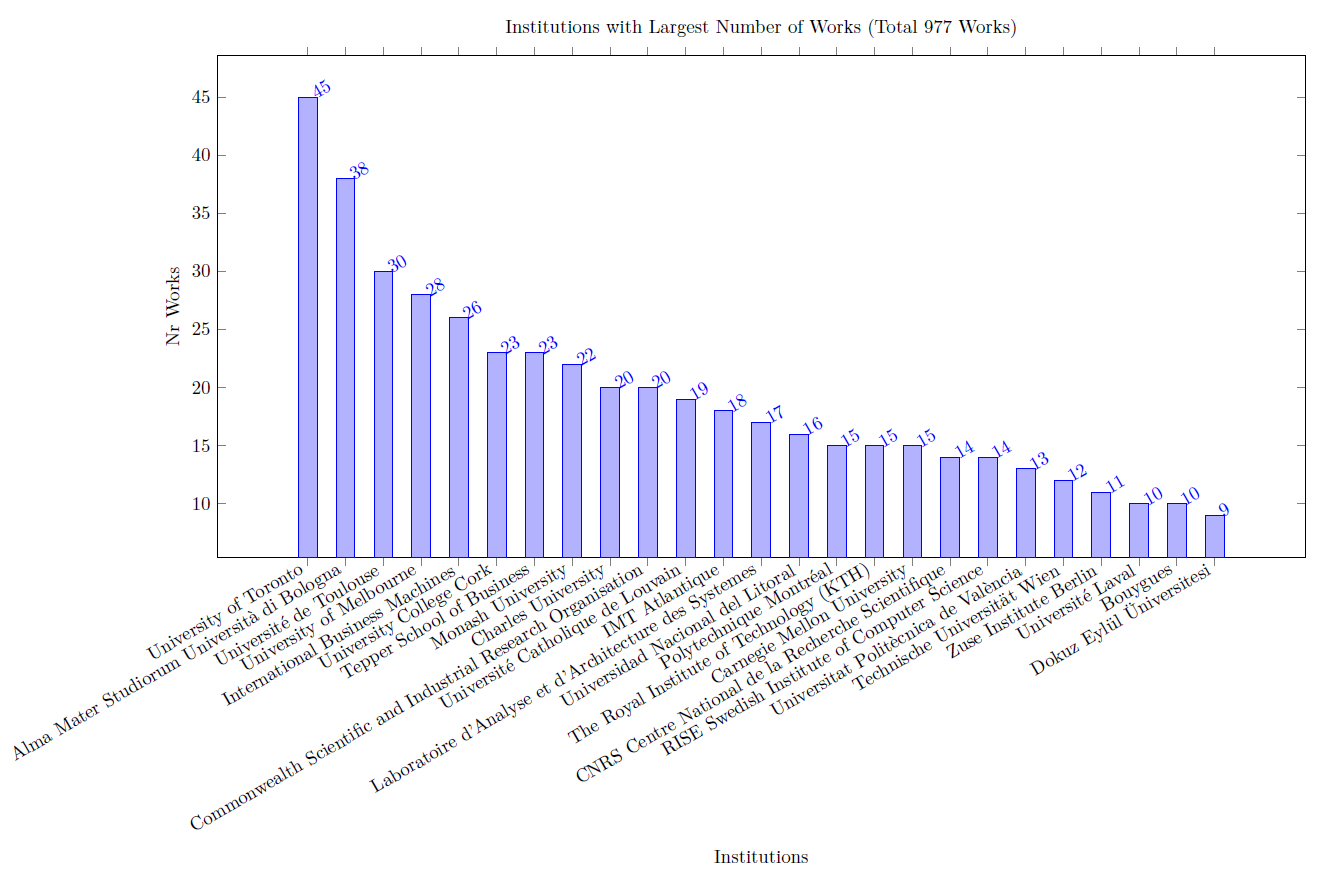
\includegraphics[width=35cm]{images/byinstitution}
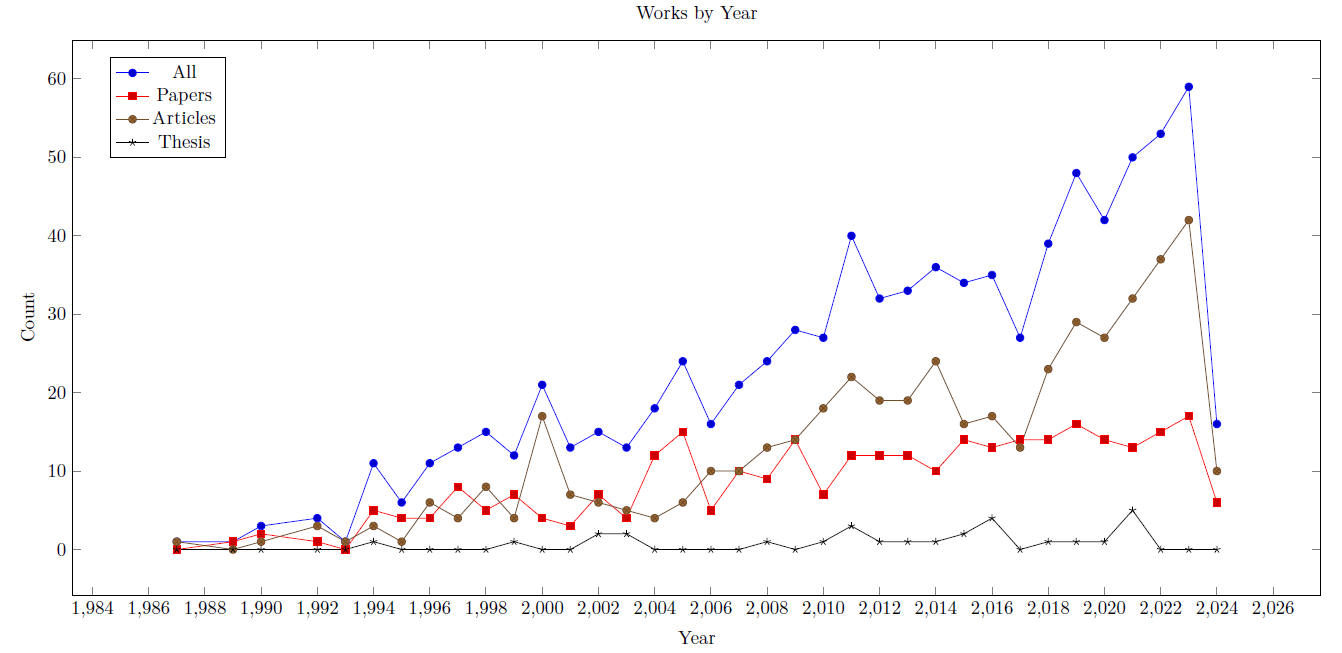
\includegraphics[width=35cm]{images/byyear}
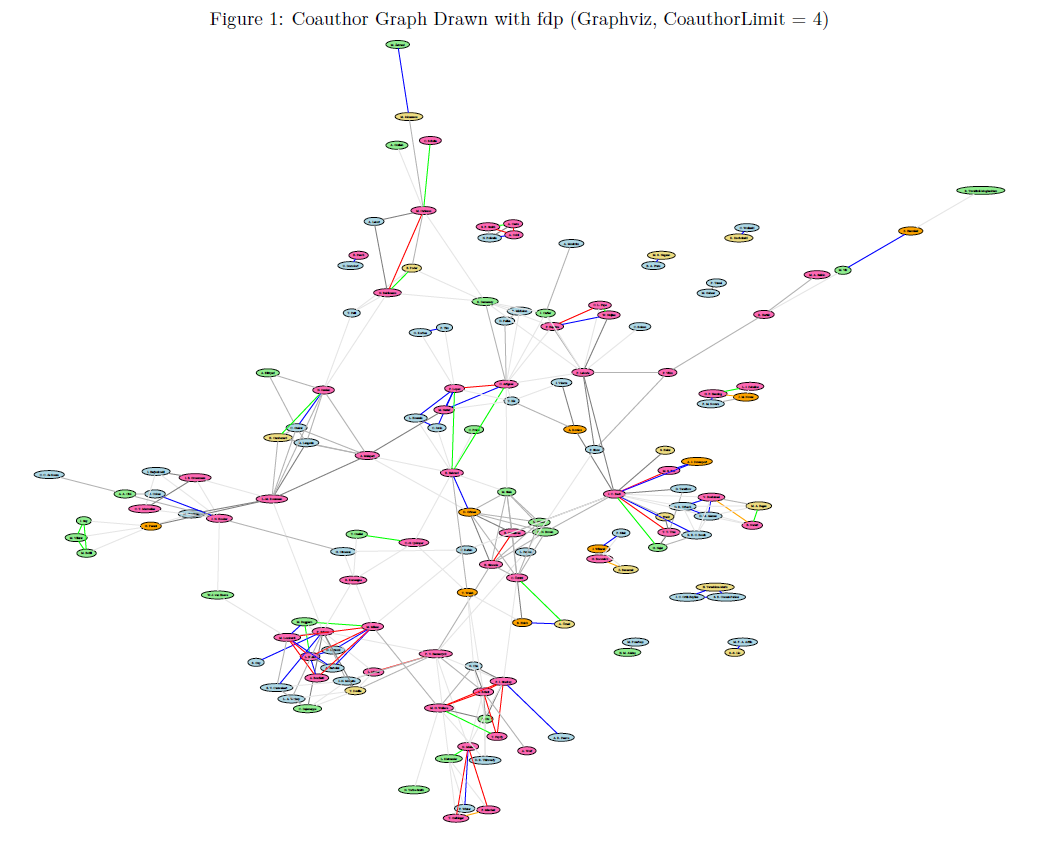
\includegraphics[width=35cm]{images/coauthorgraph}
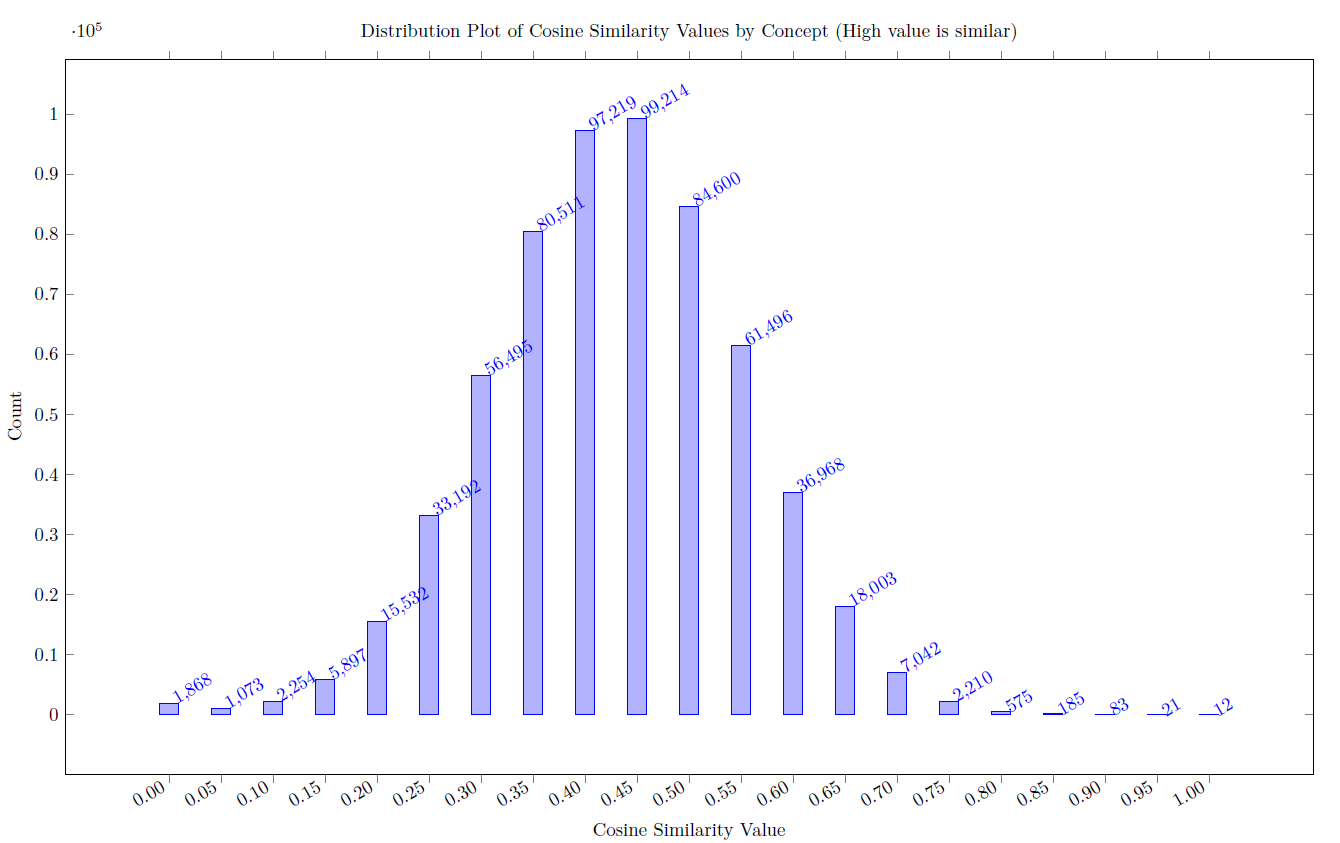
\includegraphics[width=35cm]{images/similaritydistributioncosine}

\section{Case studies}
\begin{tabular}{lllrrr}\toprule
Topic & \shortstack{Work\\With} & \shortstack{Seed\\Library} & \shortstack{Ontology\\Terms} & \shortstack{Works\\Found} & \shortstack{Works\\Considered}\\ \midrule 
CP \& Scheduling &\shortstack[l]{H. Simonis\\C. Öztürk}  & \shortstack[l]{DBLP\\223}& 407 & 1,263 & 28,313\\\midrule 
Medical \& Drones & \shortstack[l]{G. Tacadao\\B. O'Sullivan\\L. Quesada\\H. Simonis} & \shortstack[l]{WoS\\106} & 119& 495 & 14,681\\\midrule 
AI \& Counter-Terrorism & \shortstack[l]{H. Simonis\\B. O'Sullivan} & \shortstack[l]{Book\\32} & 183 & 1,603 & 75,792\\\midrule
Uncertain \& CP & \shortstack[l]{J. Lopez\\H. Simonis} & \shortstack[l]{Manual\\6} & 13 & 106 & 3,328\\
\bottomrule
\end{tabular} 

\section{Limitations}
\begin{itemize}
\item Some relevant works do not have DOI 
\begin{itemize}
\item Theses, Workshops
\item Older AI conference proceedings (before 2006)
\end{itemize}
\item No access to some journals, book chapters, books (no pdf) 
\item Identifying authors without orcid is tedious at best
\item If only the databases made all their data available
\end{itemize} 
\section{To learn more}
\begin{center}
%%%% replace as required with more specific links
\qrcode[link,height=5cm]{https://hsimonis.github.io/pthg24/scheduling/scheduling.pdf}
\end{center}

\end{multicols}
\end{frame}
\end{document}
%%%%%%%%%%%%%%%%%%%%%%%%%%%%%%%%%%%%%%%%%%%%%%%%%%%%%%%%%%%%%%%%%%%%%%%%%%%%%%